\section*{Zadanie 23.}
\begin{task}
Przedyskutować fizyczne efekty związane z prawem Faraday`a.
\end{task}

\begin{solution}
Pod wpływem zmian strumienia magnetycznego powstaje w ramce przewodzącej siła elektromotoryczna równa co do wartości szybkości zmian strumienia magnetycznego. Zwrot siły elektromotorycznej jest taki, że spowodowany przez nią prąd wywołuje pole magnetyczne przeciwstawiające się zmianom pola zewnętrzengo.
Po uwzględnieniu znaku, siła elektromotoryczna wyraża się wzorem:
$$ V = \cfrac{-\partial\varphi}{\partial t}$$
$$ V = \oint_{l}\vec{E}d\vec{l} $$
$$ \varphi = \iint_{S}\vec{B}\vec{n}ds$$
\begin{center}
$\oint_{l}\vec{E}d\vec{l}=-\iint_{S}\cfrac{\partial\vec{B}}{\partial t}\vec{n}ds $ - I równanie Maxwella\\

    $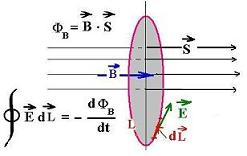
\includegraphics[scale=1]{23}$\\
    \end{center}
\end{solution}
